\documentclass[conference]{IEEEtran}
\IEEEoverridecommandlockouts

\usepackage{cite}
\usepackage{amsmath,amssymb,amsfonts}
\usepackage{algorithmic}
\usepackage{graphicx}
\usepackage{textcomp}
\usepackage{xcolor}
\usepackage{booktabs}
\usepackage{array}
\usepackage{listings}
\usepackage{url}
\usepackage{hyperref}
\usepackage{tikz}
\usepackage{pgfplots}
\pgfplotsset{compat=1.18}
\usetikzlibrary{arrows.meta, positioning, shapes.geometric, fit, backgrounds, calc, decorations.pathreplacing}

\lstset{
  basicstyle=\ttfamily\scriptsize,
  breaklines=true,
  frame=single,
  captionpos=b,
  xleftmargin=2mm,
  xrightmargin=2mm,
  aboveskip=4pt,
  belowskip=4pt
}

\hypersetup{colorlinks=true, linkcolor=blue, citecolor=blue, urlcolor=blue}

%% Color palette matching the diagram
\definecolor{nodeblue}{RGB}{52,100,160}
\definecolor{nodegold}{RGB}{180,130,30}
\definecolor{nodeteal}{RGB}{30,110,100}
\definecolor{nodepurple}{RGB}{100,60,160}
\definecolor{nodeorange}{RGB}{200,120,20}
\definecolor{nodegray}{RGB}{70,70,80}
\definecolor{lightgray}{RGB}{230,230,235}

\def\BibTeX{{\rm B\kern-.05em{\sc i\kern-.025em b}\kern-.08em T\kern-.1667em\lower.7ex\hbox{E}\kern-.125emX}}

\begin{document}

\title{FHE-402: Agentic Secret Management via\\
FHE-Protected Credentials, HMAC Key Derivation,\\
and Decentralized Proxy Validation}

\author{
\IEEEauthorblockN{FHE-402 Research Group}
\IEEEauthorblockA{Decentralized Infrastructure Division\\
\textit{Technical Specification v1.0}\\
2026}
}

\maketitle

%% -------------------------------------------------------------------
\begin{abstract}
The API credential management industry operates on a fundamentally broken trust model.
Vendors issue static bearer tokens with no cryptographic enforcement of access rules.
Rate limits, expiry, and usage constraints live in vendor databases enforced by policy,
not mathematics. A single server compromise exposes every issued credential simultaneously,
and AI agents that require plaintext secrets expose those secrets through context windows,
chat logs, and training-data pipelines.

This paper introduces \textbf{FHE-402}, the Agentic Secret Management (ASM) system: a
decentralized API access marketplace that replaces vendor trust with cryptographic guarantees.
Access tokens are derived via HMAC-SHA256 from a master key $K_m$ protected by Fully
Homomorphic Encryption (FHE) on-chain, validated offline by a Decentralized Physical
Infrastructure Network (DePIN) of proxy nodes, and bound cryptographically to the buyer's
wallet identity. Three core contributions are presented: (1) on-chain FHE storage of
$K_m$ using \texttt{euint256} with access-control-list (ACL) gating on Fhenix, (2) the
Blind Courier Protocol for cryptographically blind credential handling by AI agents, and (3)
a DePIN validation layer that eliminates single points of failure in request forwarding.

The system is post-quantum secure for the confidentiality of $K_m$ via lattice-based
TFHE, while the broader Ethereum infrastructure is not. Three open research questions are
identified and honestly characterized: FHE-friendly MAC primitive selection, symmetric
wrapping performance, and homomorphic rate-limit subdivision. The PoC implementation is
fully buildable with current tooling; the full vendor-offline architecture awaits resolution
of the MAC primitive problem.
\end{abstract}

\begin{IEEEkeywords}
Fully Homomorphic Encryption, API access control, DePIN, HMAC, AI agents, blockchain,
credential management, Fhenix, CoFHE
\end{IEEEkeywords}

%% -------------------------------------------------------------------
\section{Introduction}

API keys are the load-bearing credentials of the modern software stack. Every call
to OpenAI, Stripe, Google Maps, or any programmatic service is authenticated by a
static bearer token: a long random string that confers full access to whoever holds it.
This model has three fundamental problems at scale.

First, \textbf{credentials are durable by default}. A leaked key is valid until
manually revoked. GitHub's secret scanning service reports over 100,000 API keys
exposed in public repositories annually \cite{github_secrets}. The only remediation
is revocation and reissuance, with no forensic trail of what was accessed in the
interim.

Second, \textbf{rules live in the wrong place}. Rate limits, expiry windows, and
usage constraints exist only in vendor databases. They are enforced by policy, not
mathematics. A vendor server compromise or a dishonest vendor can silently violate
every constraint without cryptographic detection.

Third, \textbf{AI agents cannot safely handle credentials}. Autonomous agents
require plaintext secrets to call external APIs. Those secrets pass through model
context windows, memory systems, and potentially training data pipelines. There is
no cryptographic mechanism today that allows an agent to \emph{use} a credential it
\emph{cannot read}.

FHE-402 addresses all three through a composition of three well-understood primitives:
FHE for on-chain credential confidentiality, HMAC-SHA256 for offline token derivation
and validation, and a permissionless DePIN network for decentralized request forwarding.
The result is an API access layer where credentials are enforced by math, master keys are
unreadable by any party except their owner, and no single infrastructure component can
compromise the system.

The remainder of this paper is structured as follows. Section~\ref{sec:related} surveys
related work. Section~\ref{sec:arch} describes the system architecture. Section~\ref{sec:crypto}
details the cryptographic stack. Section~\ref{sec:protocol} presents the Blind Courier
Protocol. Section~\ref{sec:depin} analyzes DePIN economics. Section~\ref{sec:security}
provides a security analysis. Section~\ref{sec:agent} discusses the AI agent use case.
Section~\ref{sec:open} characterizes open research problems. Section~\ref{sec:roadmap}
outlines the implementation roadmap. Section~\ref{sec:conclusion} concludes.

%% -------------------------------------------------------------------
\section{Related Work}
\label{sec:related}

\subsection{Traditional API Gateways}
Existing API management platforms such as Kong \cite{kong} and AWS API Gateway \cite{aws_apigw}
provide rate limiting, authentication, and routing as centralized services. These systems
improve on raw static keys but retain fundamental trust assumptions: all enforcement logic
executes on vendor-controlled infrastructure, and credentials are stored in plaintext or
reversibly encrypted. A single gateway compromise exposes all managed secrets. FHE-402
replaces centralized enforcement with on-chain cryptographic rules and distributes validation
across a permissionless node network.

\subsection{Threshold Cryptography and Secret Management}
Lit Protocol \cite{lit_protocol} provides decentralized threshold key management using
multi-party computation (MPC). Users can store encrypted secrets and define conditions
under which they are decrypted. FHE-402's Threshold Services Network (TSN) component
is directly analogous in function, differing in its integration with FHE-computed tokens
and economic staking via EigenLayer. Shamir Secret Sharing \cite{shamir} provides the
theoretical foundation for threshold schemes; FHE-402 adopts an $N/2$-of-$N$ threshold
model for the TSN.

\subsection{FHE in Production Systems}
Zama's TFHE library \cite{zama_tfhe} and Fhenix \cite{fhenix} represent the
current state of the art in production-grade FHE for blockchain applications. The CoFHE
coprocessor architecture \cite{cofhe} offloads intensive FHE computation from the main
execution thread, enabling practical latencies for simple operations (addition, comparison)
while complex operations such as homomorphic MAC computation remain an open problem.
BFV \cite{bfv} complements TFHE for polynomial arithmetic workloads. FHE-402 uses TFHE
exclusively for master key storage and ACL operations.

\subsection{DePIN Economic Models}
Decentralized Physical Infrastructure Networks have demonstrated viable economic models
across several domains. Helium \cite{helium} decentralizes wireless network infrastructure;
Filecoin \cite{filecoin} decentralizes storage; Render Network \cite{render} decentralizes
GPU compute. Each demonstrates the core DePIN primitive: nodes stake collateral, provide
a measurable service, earn fees proportional to service delivered, and face slashing for
provable misbehavior. FHE-402 applies this model to API request forwarding and validation.

\subsection{Agentic Payment Protocols}
The HTTP 402 Payment Required mechanism and its modern implementation x402 \cite{x402}
enable per-request micropayments for API access. The protocol requires multiple round-trips:
agent discovers payment requirement, initiates payment, receives receipt, includes receipt
in retry, and vendor verifies payment before serving the response. For high-frequency
agentic workloads (thousands of requests per hour), this overhead is prohibitive. FHE-402
replaces per-request payment with session token issuance, bundling payment and access
proof into a single token delivery.

%% -------------------------------------------------------------------
\section{System Architecture}
\label{sec:arch}

\subsection{The Glue and Coprocessor Model}

FHE-402 follows the ``Glue and Coprocessor'' architecture. The EVM-compatible blockchain
(Fhenix) handles business logic and state management --- the ``glue'' ---
while the CoFHE Coprocessor handles intensive encrypted computations. This separation
ensures that FHE operations do not block normal contract execution and enables
horizontal scaling of the computation layer independently of the consensus layer.

\subsection{System Components}

\textbf{On-Chain Layer (Fhenix):} The on-chain layer manages encrypted state using the
\texttt{FHE.sol} library. It handles vendor registration, buyer payments in USDC,
token commitment storage via keccak256, rate limit enforcement at issuance time, and
the vendor marketplace registry.

\textbf{CoFHE Coprocessor:} A specialized, stateless engine that offloads heavy FHE
tasks from the main execution thread. Published benchmarks report significant throughput
improvements for simple FHE operations (addition, comparison). Complex operations such
as homomorphic MAC computation exhibit substantially higher latency and represent the
primary technical risk for the target architecture.

\textbf{Threshold Services Network (TSN):} A decentralized network of nodes employing
Threshold FHE Decryption and MPC Rounding \cite{mpc_rounding} to securely re-encrypt
or reveal data. The TSN operates on an $N/2$-of-$N$ trust model: no single node can
decrypt unilaterally, preventing insider attacks. Secured via EigenLayer restaking,
providing economic accountability for threshold operations.

\textbf{DePIN Proxy Network:} A permissionless network of independently operated validator
nodes positioned between API buyers and vendor endpoints. Nodes stake USDC collateral,
validate derived keys locally via HMAC recomputation without blockchain calls, forward
valid requests to vendor APIs, and earn per-request fees. This layer eliminates the
vendor proxy as a single point of failure.

\textbf{Vendor Marketplace:} An on-chain registry where vendors list APIs, pricing tiers,
and access rules. Non-custodial: funds flow directly from buyer to smart contract with
automatic distribution to vendors and nodes.

Figure~\ref{fig:arch} illustrates the complete system architecture, showing all
components and their interactions including encrypted channels, on-chain state, and the
DePIN proxy layer.

\begin{figure*}[!t]
\centering
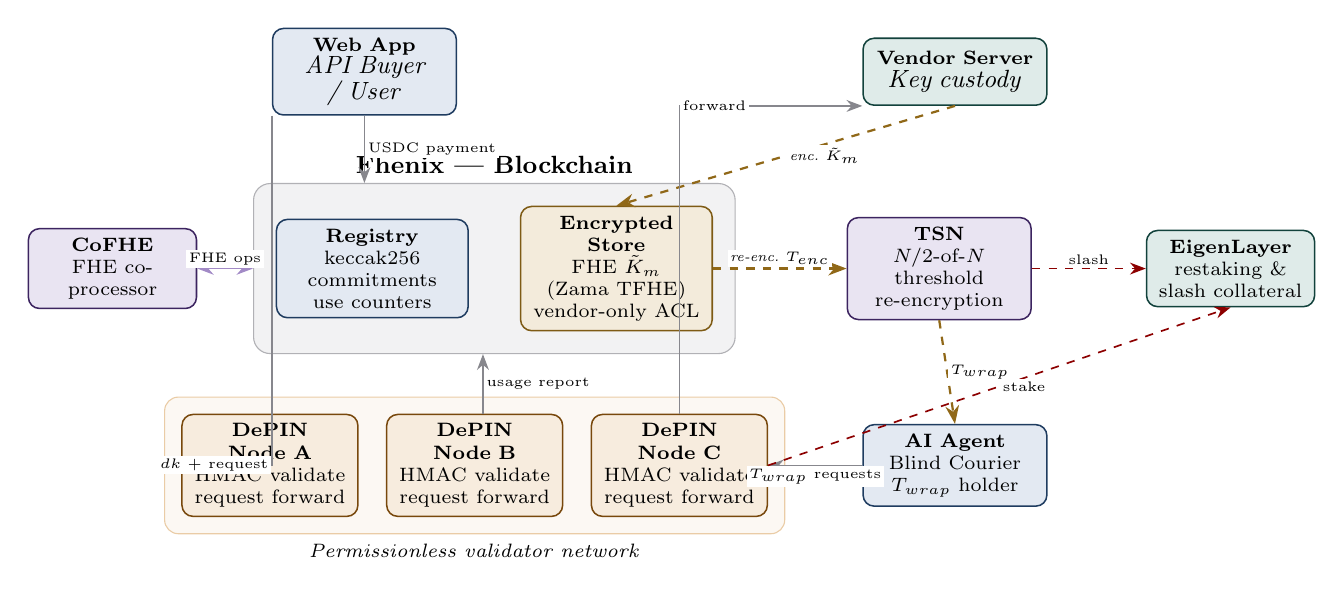
\begin{tikzpicture}[
  font=\scriptsize,
  >=Stealth,
  every node/.style={align=center},
  box/.style={draw, rounded corners=4pt, minimum width=2.1cm, minimum height=0.85cm,
              text width=2.1cm, fill=#1!14, draw=#1!60!black, line width=0.55pt},
  encbox/.style={draw, rounded corners=4pt, minimum width=2.2cm, minimum height=0.85cm,
                 text width=2.2cm, fill=nodegold!16, draw=nodegold!70!black, line width=0.55pt},
  arrlbl/.style={font=\tiny, midway, fill=white, inner sep=1pt},
  encarrow/.style={->, draw=nodegold!80!black, line width=0.8pt, dashed},
  plainarrow/.style={->, draw=nodegray!65, line width=0.6pt},
  redarrow/.style={->, draw=red!55!black, line width=0.6pt, dashed},
]

%% Row 1: Web App (x=3.5) | Vendor Server (x=11)
\node[box=nodeblue] (webapp) at (3.5, 6.8)
  {\textbf{Web App}\\\small\textit{API Buyer / User}};
\node[box=nodeteal] (vendor) at (11.0, 6.8)
  {\textbf{Vendor Server}\\\small\textit{Key custody}};

%% Row 2: CoFHE | Blockchain | TSN | EigenLayer
\node[box=nodepurple, minimum width=1.9cm, text width=1.9cm]
  (cofhe) at (0.3, 4.3)
  {\textbf{CoFHE}\\FHE coprocessor};

\node[box=nodeblue, minimum width=2.2cm, text width=2.2cm]
  (registry) at (3.6, 4.3)
  {\textbf{Registry}\\keccak256 commitments\\use counters};

\node[encbox]
  (fhestore) at (6.7, 4.3)
  {\textbf{Encrypted Store}\\FHE $\tilde{K}_m$ (Zama TFHE)\\vendor-only ACL};

\begin{scope}[on background layer]
  \node[draw=nodegray!42, fill=nodegray!7, rounded corners=6pt,
        fit=(registry)(fhestore), inner sep=8pt,
        label=above:{\small\textbf{Fhenix --- Blockchain}}]
        (chain) {};
\end{scope}

\node[box=nodepurple, minimum width=2.1cm, text width=2.1cm]
  (tsn) at (10.8, 4.3)
  {\textbf{TSN}\\$N/2$-of-$N$ threshold\\re-encryption};

\node[box=nodeteal, minimum width=1.9cm, text width=1.9cm]
  (eigen) at (14.5, 4.3)
  {\textbf{EigenLayer}\\restaking \&\\slash collateral};

%% Row 3: DePIN nodes | AI Agent
\node[box=nodeorange, minimum width=2.0cm, text width=2.0cm]
  (depin1) at (2.3, 1.8)
  {\textbf{DePIN Node A}\\HMAC validate\\request forward};
\node[box=nodeorange, minimum width=2.0cm, text width=2.0cm]
  (depin2) at (4.9, 1.8)
  {\textbf{DePIN Node B}\\HMAC validate\\request forward};
\node[box=nodeorange, minimum width=2.0cm, text width=2.0cm]
  (depin3) at (7.5, 1.8)
  {\textbf{DePIN Node C}\\HMAC validate\\request forward};

\begin{scope}[on background layer]
  \node[draw=nodeorange!38, fill=nodeorange!5, rounded corners=5pt,
        fit=(depin1)(depin2)(depin3), inner sep=6pt,
        label=below:{\scriptsize\textit{Permissionless validator network}}]
        (depingroup) {};
\end{scope}

\node[box=nodeblue, minimum width=2.1cm, text width=2.1cm]
  (agent) at (11.0, 1.8)
  {\textbf{AI Agent}\\Blind Courier\\$T_{wrap}$ holder};

%% Arrows
\draw[plainarrow] (webapp.south) -- (chain.north -| webapp.south)
  node[arrlbl, right]{USDC payment};
\draw[encarrow] (vendor.south) -- (fhestore.north)
  node[arrlbl, right]{\textit{enc.}~$\tilde{K}_m$};
\draw[<->, draw=nodepurple!60, line width=0.65pt]
  (cofhe.east) -- (chain.west)
  node[arrlbl, above]{FHE ops};
\draw[encarrow] (fhestore.east) -- (tsn.west)
  node[arrlbl, above]{\textit{re-enc.}~$T_{enc}$};
\draw[encarrow] (tsn.south) -- (agent.north)
  node[arrlbl, right]{$T_{wrap}$};
\draw[plainarrow] (webapp.south west) |- (depingroup.west |- depin1.west)
  node[arrlbl, left]{$dk$ + request};
\draw[plainarrow] ([xshift=3pt]depin2.north) -- ([xshift=3pt]chain.south -| depin2.north)
  node[arrlbl, right]{usage report};
\draw[plainarrow] (depin3.north) |- (vendor.south west)
  node[arrlbl, right]{forward};
\draw[plainarrow] (agent.west) -- (depin3.east)
  node[arrlbl, below]{$T_{wrap}$ requests};
\draw[redarrow] (depin3.east) -- (eigen.south)
  node[arrlbl, right]{\tiny stake};
\draw[redarrow] (tsn.east) -- (eigen.west)
  node[arrlbl, above]{\tiny slash};

\end{tikzpicture}
\caption{FHE-402 complete system architecture. Dashed orange arrows: encrypted channels.
Gray arrows: plaintext protocol messages. Red dashed arrows: EigenLayer staking/slashing.
$K_m$ exists only as FHE ciphertext $\tilde{K}_m$ on-chain; no party can read it in plaintext.}
\label{fig:arch}
\end{figure*}

\subsection{Comparison with Existing Solutions}

Table~\ref{tab:comparison} compares FHE-402 against traditional API keys and OAuth 2.0
across the dimensions most relevant to security and decentralization.

\begin{table}[h]
\caption{Comparison: Traditional API Keys vs. OAuth 2.0 vs. FHE-402}
\label{tab:comparison}
\renewcommand{\arraystretch}{1.2}
\begin{tabular}{p{1.6cm}p{1.7cm}p{1.7cm}p{1.9cm}}
\toprule
\textbf{Property} & \textbf{API Keys} & \textbf{OAuth 2.0} & \textbf{FHE-402} \\
\midrule
Rules enforcement & Vendor DB & Auth server & Cryptography \\
Secret location & Vendor server & Auth server & FHE on-chain \\
Key binding & None (bearer) & User session & Wallet identity \\
Validation & Network call & Network call & Local HMAC \\
SPOF & Vendor server & Auth server & None (DePIN) \\
Auditable & No & No & On-chain \\
Post-quantum & No & No & Yes ($K_m$ only) \\
\bottomrule
\end{tabular}
\end{table}

%% -------------------------------------------------------------------
\section{Cryptographic Stack}
\label{sec:crypto}

\subsection{secp256k1 (ECDSA)}
Used for vendor registration and buyer wallet binding. The vendor's Ethereum wallet
signs the registration transaction. The buyer's wallet address is embedded as an explicit
input to the HMAC derivation function, binding every derived key to a specific on-chain
identity. Standard Ethereum tooling; no custom implementation required.

\subsection{HMAC-SHA256 --- Key Derivation}
The key derivation primitive for the PoC implementation. Given master key $K_m$ and a
structured payload, the derived key is computed as:

\begin{equation}
dk = \mathrm{HMAC\text{-}SHA256}(K_m,\ W \| N \| M \| E)
\label{eq:hmac}
\end{equation}

where $W$ is the buyer's wallet address, $N$ is a cryptographically random nonce,
$M$ is the maximum use count, and $E$ is the expiry timestamp. The derived key is
deterministic: given identical inputs, the same $dk$ is produced. Inversion is
computationally infeasible: possession of $dk$ reveals nothing about $K_m$. Validation
at a DePIN node requires only the locally cached $K_m$; no network call is required.
Validation latency is sub-millisecond.

\subsection{Keccak-256 --- On-Chain Commitment}
The derived key itself never appears on-chain. Instead, its hash is recorded:

\begin{equation}
c = \mathrm{keccak256}(dk)
\label{eq:commitment}
\end{equation}

Commitment $c$ proves that key $dk$ was legitimately issued without revealing $dk$.
It also anchors the on-chain use counter: the contract increments a counter keyed by
$c$ upon each validated usage report from DePIN nodes.

\subsection{TFHE / BFV --- Master Key Encryption}
TFHE \cite{zama_tfhe} operates on binary circuits optimized for gate-by-gate operations.
BFV \cite{bfv} operates on integer arithmetic more efficiently for polynomial computations.
The master key $K_m$ is stored as \texttt{euint256}, a 256-bit encrypted integer equivalent
in security to AES-256. The FHE layer is post-quantum secure via lattice-based cryptography.

The ECDSA layer (wallet signatures, EigenLayer) is \emph{not} post-quantum secure. The
post-quantum property applies specifically to the confidentiality of encrypted on-chain state.

\subsection{Homomorphic MAC (Open Research)}
The MAC primitive for on-chain token generation must be TFHE-compatible. Standard
constructions are incompatible: Poseidon hash is designed for ZK-SNARK prime-field
arithmetic and maps poorly to TFHE's binary circuits; its round function involves
field exponentiations that are prohibitively expensive in binary gate representation.
HMAC-SHA256 similarly requires bitwise operations at a scale that exceeds current
CoFHE throughput for interactive workloads. Candidate FHE-native alternatives include
LowMC \cite{lowmc}, Kreyvium \cite{kreyvium}, and custom constructions based on
TFHE-native integer addition, multiplication, and bitwise operations. The selection
of a suitable MAC primitive is an \textbf{open research question} (see Section~\ref{sec:open}).

\subsection{Symmetric Wrapping (Open Research)}
Converting FHE-encrypted tokens into standard symmetric ciphertext for delivery requires
trans-ciphering: computing AES decryption inside the FHE circuit. AES trans-ciphering
under TFHE is prohibitively expensive at current performance levels (minutes per token).
FHE-friendly alternatives include Pasta \cite{pasta} and Elisabeth \cite{elisabeth},
designed for efficient homomorphic evaluation. Practical latency benchmarks for these
candidates on CoFHE hardware are required (see Section~\ref{sec:open}).

Table~\ref{tab:primitives} summarizes the role and status of each primitive.

\begin{table}[h]
\caption{Cryptographic Primitive Responsibilities}
\label{tab:primitives}
\renewcommand{\arraystretch}{1.2}
\begin{tabular}{p{1.8cm}p{2.0cm}p{2.2cm}}
\toprule
\textbf{Primitive} & \textbf{Role} & \textbf{Status} \\
\midrule
secp256k1 & Wallet binding & Production ready \\
HMAC-SHA256 & Key derivation, validation & Production ready \\
Keccak-256 & On-chain commitment & Production ready \\
TFHE/euint256 & $K_m$ storage \& ACL & Production ready \\
Homomorphic MAC & On-chain token gen. & Open research \\
Symmetric wrap & Token delivery & Open research \\
\bottomrule
\end{tabular}
\end{table}

%% -------------------------------------------------------------------
\section{Protocol Design: The Blind Courier Protocol}
\label{sec:protocol}

\subsection{The Blind Courier Abstraction}
The system treats the AI agent as a Blind Courier. The agent receives an Access Token
encrypted specifically for the Service Vendor. The agent can forward this token to
prove permission to use a service but cannot decrypt it to recover the underlying
secret. This property is enforced by cryptography, not policy: the token is encrypted
under the vendor's public key via the TSN. No amount of memory inspection or model
introspection allows the agent to recover $K_m$.

Figure~\ref{fig:protocol} shows the complete four-phase protocol flow with all
participating actors and message types.

\begin{figure*}[!t]
\centering
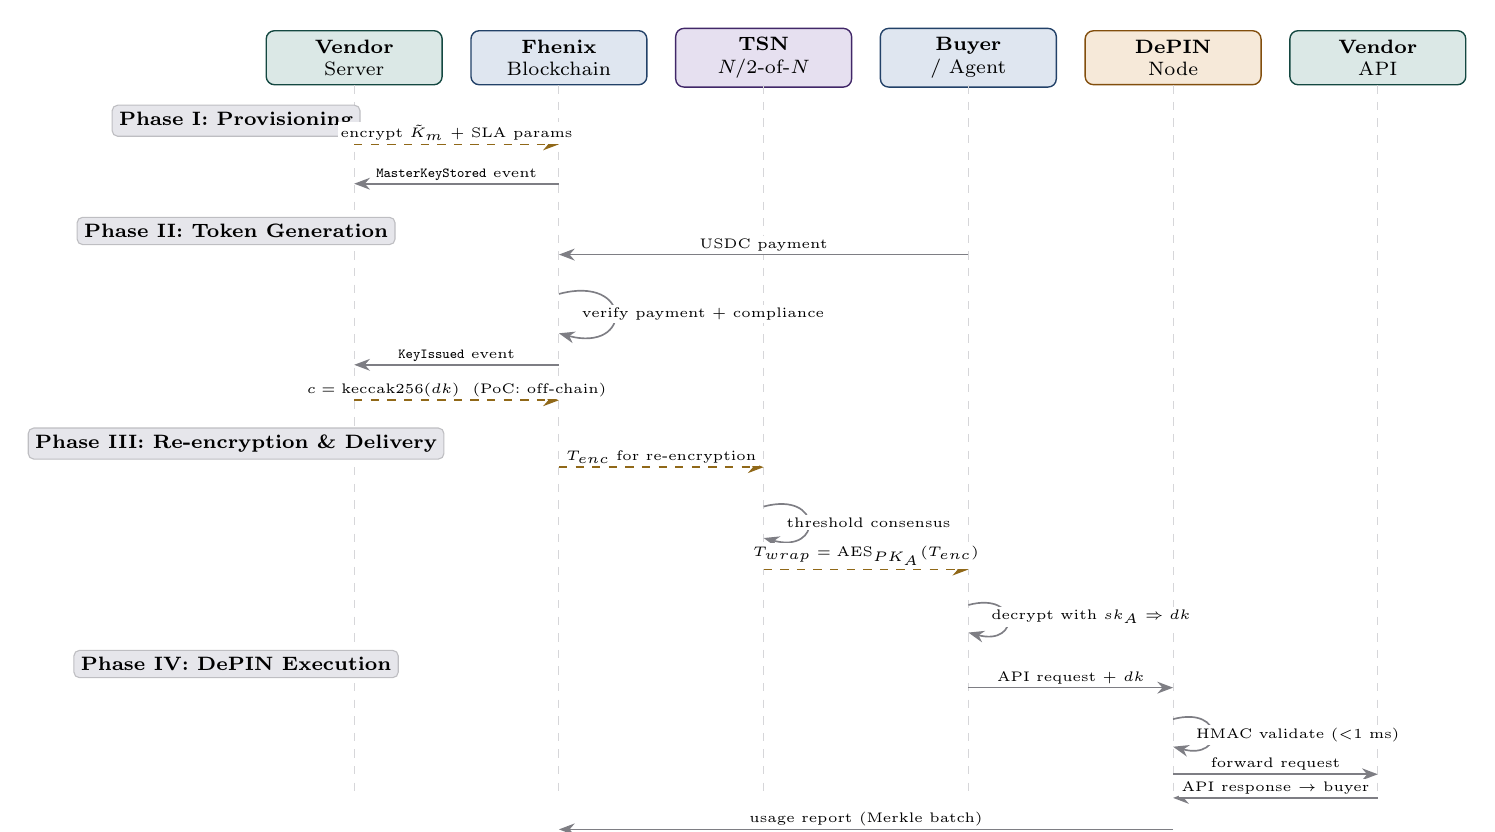
\begin{tikzpicture}[
  font=\scriptsize,
  >=Stealth,
  every node/.style={align=center},
  actorbox/.style={draw, rounded corners=3pt, fill=#1!16, draw=#1!65!black,
                   minimum width=2.0cm, minimum height=0.6cm, text width=2.0cm,
                   line width=0.5pt},
  msg/.style={->, draw=nodegray!70, line width=0.6pt},
  emsg/.style={->, draw=nodegold!80!black, line width=0.6pt, dashed},
  phaselbl/.style={draw=nodegray!35, fill=lightgray, rounded corners=2pt,
                   inner sep=2.5pt, font=\scriptsize\bfseries},
  steplbl/.style={font=\tiny, fill=white, inner sep=1pt},
]

%% Actor x-positions (2.6cm spacing -> 5*2.6 = 13cm span)
\def\xA{0}      % Vendor Server
\def\xB{2.6}    % Fhenix
\def\xC{5.2}    % TSN
\def\xD{7.8}    % Buyer / Agent
\def\xE{10.4}   % DePIN Node
\def\xF{13.0}   % Vendor API

%% Actor header boxes at y=0
\node[actorbox=nodeteal]   at (\xA,0) {\textbf{Vendor}\\Server};
\node[actorbox=nodeblue]   at (\xB,0) {\textbf{Fhenix}\\Blockchain};
\node[actorbox=nodepurple] at (\xC,0) {\textbf{TSN}\\$N/2$-of-$N$};
\node[actorbox=nodeblue]   at (\xD,0) {\textbf{Buyer}\\/ Agent};
\node[actorbox=nodeorange] at (\xE,0) {\textbf{DePIN}\\Node};
\node[actorbox=nodeteal]   at (\xF,0) {\textbf{Vendor}\\API};

%% Lifelines
\foreach \x in {\xA,\xB,\xC,\xD,\xE,\xF}{
  \draw[draw=nodegray!22, line width=0.35pt, dashed] (\x,-0.35) -- (\x,-9.4);
}

%% ---- PHASE I: Provisioning ----
\node[phaselbl] at (-1.5,-0.8) {Phase I: Provisioning};
\draw[emsg] (\xA,-1.1) -- (\xB,-1.1)
  node[steplbl,above,midway]{encrypt $\tilde{K}_m$ + SLA params};
\draw[msg,<-] (\xA,-1.6) -- (\xB,-1.6)
  node[steplbl,above,midway]{\texttt{MasterKeyStored} event};

%% ---- PHASE II: Token Generation ----
\node[phaselbl] at (-1.5,-2.2) {Phase II: Token Generation};
\draw[msg] (\xD,-2.5) -- (\xB,-2.5)
  node[steplbl,above,midway]{USDC payment};
\draw[msg] (\xB,-3.0) to[out=15,in=-15,looseness=5] (\xB,-3.5);
\node[steplbl,right] at (\xB+0.25,-3.25) {verify payment + compliance};
\draw[msg] (\xB,-3.9) -- (\xA,-3.9)
  node[steplbl,above,midway]{\texttt{KeyIssued} event};
\draw[emsg] (\xA,-4.35) -- (\xB,-4.35)
  node[steplbl,above,midway]{$c=\mathrm{keccak256}(dk)$\ \ (PoC: off-chain)};

%% ---- PHASE III: Re-encryption & Delivery ----
\node[phaselbl] at (-1.5,-4.9) {Phase III: Re-encryption \& Delivery};
\draw[emsg] (\xB,-5.2) -- (\xC,-5.2)
  node[steplbl,above,midway]{$T_{enc}$ for re-encryption};
\draw[msg] (\xC,-5.7) to[out=15,in=-15,looseness=5] (\xC,-6.1);
\node[steplbl,right] at (\xC+0.25,-5.9) {threshold consensus};
\draw[emsg] (\xC,-6.5) -- (\xD,-6.5)
  node[steplbl,above,midway]{$T_{wrap}=\mathrm{AES}_{PK_A}(T_{enc})$};
\draw[msg] (\xD,-6.95) to[out=15,in=-15,looseness=5] (\xD,-7.3);
\node[steplbl,right] at (\xD+0.25,-7.1) {decrypt with $sk_A \Rightarrow dk$};

%% ---- PHASE IV: DePIN Execution ----
\node[phaselbl] at (-1.5,-7.7) {Phase IV: DePIN Execution};
\draw[msg] (\xD,-8.0) -- (\xE,-8.0)
  node[steplbl,above,midway]{API request $+$ $dk$};
\draw[msg] (\xE,-8.4) to[out=15,in=-15,looseness=5] (\xE,-8.75);
\node[steplbl,right] at (\xE+0.25,-8.6) {HMAC validate ($<$1 ms)};
\draw[msg] (\xE,-9.1) -- (\xF,-9.1)
  node[steplbl,above,midway]{forward request};
\draw[msg] (\xF,-9.4) -- (\xE,-9.4)
  node[steplbl,above,midway]{API response $\rightarrow$ buyer};
\draw[msg,transform canvas={yshift=-0.4cm}] (\xE,-9.4) -- (\xB,-9.4)
  node[steplbl,above,midway]{usage report (Merkle batch)};

\end{tikzpicture}
\caption{Blind Courier Protocol: four-phase message sequence across all six participants.
Dashed orange: encrypted payloads. Gray: plaintext messages. Looped arrows: internal
processing (no network hop). Phase II commitment delivery is vendor-mediated in the PoC;
the Phase 2 roadmap replaces this with trustless on-chain CoFHE computation.}
\label{fig:protocol}
\end{figure*}

\subsection{Phase I: Provisioning}
The vendor generates $K_m$ locally on a secured system. $K_m$ is encrypted client-side
using the Fhenix FHE public key, producing a ciphertext $\tilde{K}_m$. The vendor
submits $\tilde{K}_m$ to the smart contract along with SLA parameters: pricing tiers,
TTL ranges, rate limits, and compliance gate specifications. After this step, the vendor's
server is not required for token issuance in the target architecture.

\subsection{Phase II: Token Generation}
The buyer (or AI agent on behalf of a user) submits payment in USDC to the smart contract.
The contract verifies payment, evaluates compliance rules against encrypted identity
attestations, and invokes the CoFHE coprocessor to compute:

\begin{equation}
T_{enc} = \mathrm{TFHE\text{-}MAC}(K_m,\ W \| N \| M \| E)
\label{eq:token}
\end{equation}

where $T_{enc}$ is an encrypted token ciphertext. In the PoC, this step is performed
off-chain by the vendor server following detection of a \texttt{KeyIssued} event.

\subsection{Phase III: Re-encryption and Delivery}
The encrypted token $T_{enc}$ is submitted to the TSN for re-encryption under the
buyer's public key $PK_A$. The TSN, operating under $N/2$-of-$N$ threshold consensus,
produces $T_{wrap} = \mathrm{AES\text{-}GCM}_{PK_A}(T_{enc})$. The buyer receives
$T_{wrap}$; decryption with their private key recovers the Access Key. No TSN node
sees the plaintext token at any point.

\subsection{Phase IV: DePIN Execution}
The buyer includes the Access Key in the HTTP \texttt{Authorization: Bearer} header
of every API request. DePIN nodes receive the request and perform local HMAC validation:

\begin{enumerate}
\item Recompute $dk' = \mathrm{HMAC\text{-}SHA256}(K_m, W \| N \| M \| E)$ using
      cached $K_m$
\item Verify $dk' = dk$ (token integrity)
\item Verify $\mathrm{timestamp} < E$ (not expired)
\item Verify $N \notin \mathcal{S}_{seen}$ (replay prevention)
\item If $M$-bounded: verify on-chain counter $< M$
\end{enumerate}

Valid requests are forwarded to the vendor API endpoint. Responses are returned to the
buyer. The node submits a signed usage report to the chain and claims its fee allocation.

\subsection{Nonce Management}
Nonces are random (not sequential) to avoid the serialization bottleneck of maintaining
a monotonic encrypted counter under FHE. The vendor maintains a time-bucketed bloom
filter for seen-nonce tracking. Two bloom filters represent the current and previous TTL
window. On each request, both are checked. At each TTL boundary, the oldest is discarded
and a fresh filter is initialized. Memory usage is bounded at $O(\lambda \cdot r_{TTL})$
where $\lambda$ is the target false-positive rate and $r_{TTL}$ is the expected request
count per TTL window.

\subsection{Rate Limit Enforcement}
Rate limits are enforced through a hybrid model:

\textbf{At issuance (on-chain):} The contract tracks total tokens issued per subscription
period. Over-issuance is prevented at the protocol level.

\textbf{At validation (off-chain):} DePIN nodes track per-token usage locally. Usage
reports are aggregated in Merkle rollups and submitted in batches to minimize gas costs.

Rate limits are \emph{advisory} at the per-request level and \emph{enforced} at the
issuance level. Per-request on-chain enforcement is infeasible; issuance-time gating
bounds total access.

\subsection{Worked Example: 10-Use Token Lifecycle}
Consider a buyer purchasing a 10-use token with nonce $N = \texttt{0xA3F2}$ and expiry
$E = t + 3600$. Table~\ref{tab:lifecycle} traces the state at key points.

\begin{table}[h]
\caption{Token Lifecycle: 10-Use Token}
\label{tab:lifecycle}
\renewcommand{\arraystretch}{1.2}
\begin{tabular}{p{1.2cm}p{1.8cm}p{1.5cm}p{1.5cm}}
\toprule
\textbf{Call} & \textbf{Nonce check} & \textbf{Counter} & \textbf{Result} \\
\midrule
1 & $N \notin \mathcal{S}$ & 1 / 10 & \textsc{forward} \\
5 & $N \notin \mathcal{S}$ & 5 / 10 & \textsc{forward} \\
10 & $N \notin \mathcal{S}$ & 10 / 10 & \textsc{forward} \\
11 & --- & 10 / 10 & \textsc{reject} (limit) \\
--- & $N \in \mathcal{S}$ & --- & \textsc{reject} (replay) \\
\bottomrule
\end{tabular}
\end{table}

On the 11th call, the counter check fails and the request is rejected with HTTP 429
before it reaches the vendor endpoint. This rejection is provable on-chain via the
committed use counter.

%% -------------------------------------------------------------------
\section{DePIN Economics}
\label{sec:depin}

\subsection{Node Registration and Staking}
Any party may join the validator network by submitting the minimum stake $S_{min}$
in USDC and deploying the open-source node software. Stake is locked in the
smart contract and subject to slashing. Figure~\ref{fig:depinflow} illustrates the
full lifecycle of a DePIN node from registration through request validation to
fee settlement.

\begin{figure}[!t]
\centering
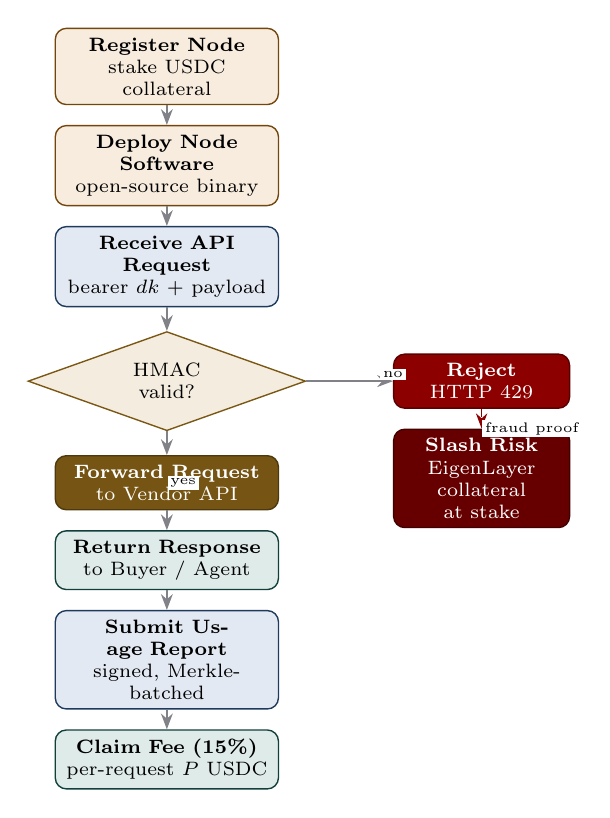
\begin{tikzpicture}[
  font=\scriptsize,
  >=Stealth,
  every node/.style={align=center},
  step/.style={draw, rounded corners=4pt, fill=#1!14, draw=#1!58!black,
               minimum width=2.6cm, minimum height=0.6cm,
               text width=2.6cm, line width=0.5pt},
  decision/.style={draw, diamond, fill=nodegold!14, draw=nodegold!68!black,
                   aspect=2.8, minimum width=2.8cm, minimum height=0.5cm,
                   text width=2.0cm, inner sep=1pt, line width=0.5pt},
  arr/.style={->, draw=nodegray!68, line width=0.6pt},
  rarr/.style={->, draw=red!55!black, line width=0.55pt, dashed},
  lbl/.style={font=\tiny, fill=white, inner sep=1pt},
]

%% Main flow at x=0, reject branch at x=3.2
\node[step=nodeorange] (reg)  at (0, 0)
  {\textbf{Register Node}\\stake USDC collateral};
\node[step=nodeorange, below=0.25cm of reg] (sw)
  {\textbf{Deploy Node Software}\\open-source binary};
\node[step=nodeblue, below=0.25cm of sw] (recv)
  {\textbf{Receive API Request}\\bearer $dk$ + payload};
\node[decision, below=0.3cm of recv] (hmac)
  {HMAC\\valid?};
\node[step=nodegold!75!black, text=white, fill=nodegold!65!black,
      below=0.3cm of hmac] (fwd)
  {\textbf{Forward Request}\\to Vendor API};
\node[step=nodeteal, below=0.25cm of fwd] (rsp)
  {\textbf{Return Response}\\to Buyer / Agent};
\node[step=nodeblue, below=0.25cm of rsp] (rep)
  {\textbf{Submit Usage Report}\\signed, Merkle-batched};
\node[step=nodeteal, below=0.25cm of rep] (fee)
  {\textbf{Claim Fee (15\%)}\\per-request $P$ USDC};

%% Reject branch (right)
\node[step=red!60!black, text=white, fill=red!55!black,
      right=1.1cm of hmac, minimum width=2.0cm, text width=2.0cm] (rej)
  {\textbf{Reject}\\HTTP 429};
\node[step=red!45!black, text=white, fill=red!40!black,
      below=0.25cm of rej, minimum width=2.0cm, text width=2.0cm] (slash)
  {\textbf{Slash Risk}\\EigenLayer\\collateral at stake};

%% Arrows: main flow
\draw[arr] (reg)  -- (sw);
\draw[arr] (sw)   -- (recv);
\draw[arr] (recv) -- (hmac);
\draw[arr] (hmac) -- (fwd)  node[lbl, right]{yes};
\draw[arr] (fwd)  -- (rsp);
\draw[arr] (rsp)  -- (rep);
\draw[arr] (rep)  -- (fee);

%% Arrows: reject branch
\draw[arr] (hmac.east) -- (rej.west) node[lbl, above]{no};
\draw[rarr] (rej.south) -- (slash.north)
  node[lbl, right]{\tiny fraud proof};

\end{tikzpicture}
\caption{DePIN node request lifecycle. Main path proceeds vertically; invalid tokens
branch right to rejection and slashing. All HMAC validation runs locally from the
cached $K_m$: no blockchain call is required per request ($<$1 ms latency).}
\label{fig:depinflow}
\end{figure}

\begin{lstlisting}[language={}, caption={Node Registration and Slashing}]
function registerNode(uint256 stakeAmount) external {
    require(stakeAmount >= MIN_STAKE,
            "insufficient stake");
    usdc.transferFrom(msg.sender,
                      address(this), stakeAmount);
    nodeStakes[msg.sender] = stakeAmount;
    emit NodeRegistered(msg.sender, stakeAmount);
}

function slashNode(address node,
    bytes calldata proof) external onlyGovernance {
    uint256 stake = nodeStakes[node];
    nodeStakes[node] = 0;
    emit NodeSlashed(node, stake);
}
\end{lstlisting}

\subsection{Fee Distribution}
Every processed request triggers a micro-payment from the pre-paid buyer allocation.
For a request priced at $P$ USDC, the distribution follows the structure shown in
Figure~\ref{fig:feedist} and Table~\ref{tab:fees}.

\begin{figure}[!t]
\centering
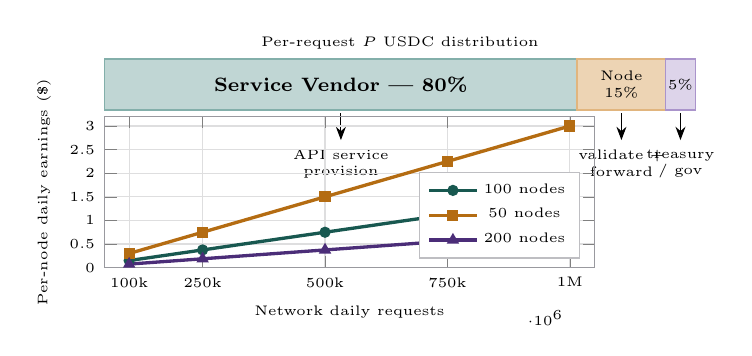
\begin{tikzpicture}[font=\scriptsize, >=Stealth]

%% Stacked bar: fee split (total width = \linewidth equivalent in TikZ = 7.5)
\def\Bw{7.5}
\def\Bh{0.65}

\fill[nodeteal!28, draw=nodeteal!55, line width=0.5pt]
  (0,0) rectangle (0.80*\Bw, \Bh);
\fill[nodeorange!32, draw=nodeorange!55, line width=0.5pt]
  (0.80*\Bw,0) rectangle (0.95*\Bw, \Bh);
\fill[nodepurple!22, draw=nodepurple!55, line width=0.5pt]
  (0.95*\Bw,0) rectangle (\Bw, \Bh);

\node[font=\scriptsize\bfseries] at (0.40*\Bw, \Bh/2)
  {Service Vendor --- 80\%};
\node[font=\tiny, align=center] at (0.875*\Bw, \Bh/2) {Node\\15\%};
\node[font=\tiny] at (0.975*\Bw, \Bh/2) {5\%};

\draw[->] (0.40*\Bw,-0.04) -- (0.40*\Bw,-0.38)
  node[below, font=\tiny, align=center]{API service\\provision};
\draw[->] (0.875*\Bw,-0.04) -- (0.875*\Bw,-0.38)
  node[below, font=\tiny, align=center]{validate +\\forward};
\draw[->] (0.975*\Bw,-0.04) -- (0.975*\Bw,-0.38)
  node[below, font=\tiny, align=center]{treasury\\/ gov};

\node[font=\tiny, above] at (\Bw/2, \Bh)
  {Per-request $P$ USDC distribution};

%% pgfplots bar chart below
\begin{scope}[yshift=-2.0cm]
\begin{axis}[
  width=7.8cm, height=3.5cm,
  xlabel={\tiny Network daily requests},
  ylabel={\tiny Per-node daily earnings (\$)},
  xtick={100000,250000,500000,750000,1000000},
  xticklabels={100k,250k,500k,750k,1M},
  ytick={0,0.5,1,1.5,2,2.5,3},
  ymin=0, ymax=3.2,
  xmin=50000, xmax=1050000,
  tick label style={font=\tiny},
  label style={font=\tiny},
  grid=major,
  grid style={draw=nodegray!18},
  axis line style={draw=nodegray!55},
  every axis plot/.append style={line width=1.2pt},
  legend style={font=\tiny, at={(0.97,0.06)}, anchor=south east,
                fill=white, draw=nodegray!35},
]
\addplot[color=nodeteal!80!black, mark=*, mark size=1.4pt]
  coordinates {(100000,0.15)(250000,0.375)(500000,0.75)(750000,1.125)(1000000,1.5)};
\addlegendentry{100 nodes};
\addplot[color=nodeorange!90!black, mark=square*, mark size=1.4pt]
  coordinates {(100000,0.30)(250000,0.75)(500000,1.5)(750000,2.25)(1000000,3.0)};
\addlegendentry{50 nodes};
\addplot[color=nodepurple!75!black, mark=triangle*, mark size=1.4pt]
  coordinates {(100000,0.075)(250000,0.1875)(500000,0.375)(750000,0.5625)(1000000,0.75)};
\addlegendentry{200 nodes};
\end{axis}
\end{scope}

\end{tikzpicture}
\caption{Top: per-request USDC fee distribution at \$0.001/call.
Bottom: per-node daily earnings vs.\ total network request volume for three node-count
scenarios (\$0.001/request, 15\% node share). At 1M daily requests with 50 nodes,
annualized yield exceeds 200\% of the \$500 minimum stake.}
\label{fig:feedist}
\end{figure}

\begin{table}[h]
\caption{Fee Distribution per Request}
\label{tab:fees}
\renewcommand{\arraystretch}{1.2}
\begin{tabular}{lll}
\toprule
\textbf{Recipient} & \textbf{Share} & \textbf{Rationale} \\
\midrule
Service Vendor & 80\% & API service provision \\
DePIN Node & 15\% & Validation + forwarding \\
Protocol Treasury & 5\% & Development, governance \\
\bottomrule
\end{tabular}
\end{table}

\subsection{Node Economics: Worked Example}
Consider a network handling 1,000,000 requests per day at \$0.001 per request,
distributed across 100 nodes of equal throughput:

\begin{align}
\text{Daily network revenue} &= 1{,}000{,}000 \times \$0.001 = \$1{,}000 \\
\text{Node share (15\%)} &= \$150 \text{ per day (network total)} \\
\text{Per-node daily earnings} &= \$150 / 100 = \$1.50 \\
\text{Annualized per node} &\approx \$547.50
\end{align}

At a minimum stake of \$500 USDC, annual yield is approximately 109\%. As network
usage scales, per-node earnings scale linearly assuming constant node count, creating
natural incentive for network growth.

\subsection{Slashing Conditions}
Nodes face slashing for provable misbehavior:
\begin{itemize}
\item \textbf{Dropped requests:} Buyer receives no response but node claims fee.
      Detectable via signed request receipts and buyer complaint.
\item \textbf{Invalid validation:} Node forwards a request with an invalid derived key.
      Detectable via on-chain commitment mismatch.
\item \textbf{TSN collusion:} Node participates in unauthorized decryption.
      Detectable via threshold cryptography proofs.
\end{itemize}

%% -------------------------------------------------------------------
\section{Security Analysis}
\label{sec:security}

\subsection{Threats Addressed}

\textbf{Credential theft at rest:} FHE encryption ensures $K_m$ has no plaintext
representation on-chain. A complete blockchain state dump reveals only the ciphertext
$\tilde{K}_m$, which is computationally indistinguishable from random under the
TFHE security assumption.

\textbf{Credential theft in transit:} Key delivery via TSN re-encryption wraps the
Access Token specifically for the buyer's public key. Only the buyer's private key
can unwrap it. No TSN node observes the plaintext token.

\textbf{Replay attacks:} Random nonces embedded in every token, combined with
vendor-side bloom filter tracking, prevent replaying captured valid requests.

\textbf{Over-issuance:} On-chain rate limits at issuance time prevent any party
from issuing tokens beyond the subscription quota, even in the event of a compromised
vendor server.

\textbf{Proxy node collusion:} EigenLayer staking combined with $N/2$-of-$N$
threshold trust for the TSN requires a majority of nodes to collude simultaneously
to break security guarantees. This is economically irrational given slashing.

\textbf{Bearer token sharing:} Wallet-bound key derivation (Equation~\ref{eq:hmac}
embeds $W$ as an HMAC input) means a derived key for wallet $W_A$ is invalid when
presented from wallet $W_B$. The keys cannot be usefully transferred.

\subsection{Threats Not Addressed}

\textbf{Vendor machine compromise:} If an attacker compromises the vendor's local
system holding $K_m$, all derived keys can be forged. FHE protects $K_m$ from
all parties \emph{except} the vendor. This is a deliberate design choice: the vendor
must trust their own infrastructure for key custody.

\textbf{Majority TSN collusion:} Compromise of more than $N/2$ TSN nodes simultaneously
allows unauthorized decryption. EigenLayer staking makes this economically costly but
not cryptographically impossible.

\textbf{Quantum attacks on ECDSA:} The Ethereum wallet layer (secp256k1 signatures,
EigenLayer restaking) is not post-quantum secure. A sufficiently capable quantum
adversary could forge wallet signatures. The FHE layer's lattice-based security
is unaffected.

\subsection{Trust Assumptions (Enumerated)}
\begin{enumerate}
\item Vendor's local key custody system is not compromised.
\item Fewer than $N/2$ TSN nodes collude at any time.
\item The Fhenix blockchain consensus mechanism is not captured.
\item EigenLayer staking provides sufficient economic deterrence for node misbehavior.
\item TFHE security reduces to the hardness of RLWE (Ring Learning With Errors).
\end{enumerate}

%% -------------------------------------------------------------------
\section{The AI Agent Use Case}
\label{sec:agent}

\subsection{The Goldfish Bowl Problem}
Traditional blockchains are fully transparent. Every state variable is public. Storing
API master keys, private SLA terms, or sensitive business logic on-chain exposes them
to every blockchain observer, competitor, and attacker simultaneously. Off-chain key
management services address transparency but reintroduce centralized trust. The
``Goldfish Bowl'' problem is the impossibility of maintaining secret state in a
trustless transparent environment without cryptographic tools. FHE solves this:
$\tilde{K}_m$ is public; $K_m$ is not.

\subsection{Blind Credential Handling}
An AI agent acting as a Blind Courier can call a paid API without its operator ever
knowing which credential was used. The agent receives $T_{wrap}$, forwards it in the
\texttt{Authorization} header, and receives the API response. It cannot inspect the
token contents. It cannot extract $K_m$. It cannot forge additional tokens.

This enables organizational delegation at scale: a company can grant an agent framework
access to 50 different vendor APIs, with each credential independently gated by
on-chain SLA rules, without exposing any credential to the agent developer.

\subsection{Compliance Gating}
The system supports compound identity checks on encrypted inputs before token issuance.
A vendor may specify: ``issue tokens only to wallets with a Self Protocol KYC proof,
from non-sanctioned jurisdictions, with an on-chain reputation score above threshold.''
All checks execute on encrypted identity attestations using FHE comparisons. The rule
produces a boolean result without any plaintext identity data touching the chain or
being visible to the vendor.

\subsection{One-Step Payment vs. x402}
Table~\ref{tab:payment} compares FHE-402 session tokens against the x402 per-request
payment protocol for a workload of 1,000 API calls.

\begin{table}[h]
\caption{Payment Model Comparison: 1,000 API Calls}
\label{tab:payment}
\renewcommand{\arraystretch}{1.2}
\begin{tabular}{lll}
\toprule
\textbf{Property} & \textbf{x402} & \textbf{FHE-402} \\
\midrule
Round-trips per call & 3--4 & 1 \\
On-chain txns & 1,000 & 1 (issuance) \\
Gas cost & $1000 \times g$ & $g$ \\
Payment latency & Per-request & Pre-paid \\
Credential exposure & Per-request & Never \\
Offline validation & No & Yes \\
\bottomrule
\end{tabular}
\end{table}

%% -------------------------------------------------------------------
\section{Open Research Problems}
\label{sec:open}

\subsection{FHE-Friendly MAC Primitive Selection}

\textbf{The problem:} On-chain token generation (Equation~\ref{eq:token}) requires
a MAC computable inside TFHE's binary circuit model. Standard MACs are incompatible:
HMAC-SHA256 requires bit-level operations at a scale that exceeds practical FHE
circuit depth; Poseidon hash uses field exponentiations that map poorly to binary gates.

\textbf{Why it matters:} Solving this enables the full target architecture where the
vendor is completely offline after provisioning. Token issuance becomes trustless,
non-interactive, and 24/7 without vendor availability.

\textbf{Candidates:}
\begin{itemize}
\item \textbf{LowMC} \cite{lowmc}: Designed to minimize AND-gate depth in circuits,
      making it FHE-friendly. Security proofs exist; no production TFHE implementation
      is publicly available as of this writing.
\item \textbf{Kreyvium} \cite{kreyvium}: A stream cipher variant of Trivium designed
      for FHE evaluation. Lower circuit depth than AES; full MAC construction requires
      additional design.
\item \textbf{Custom TFHE constructions}: Integer addition and multiplication chains
      native to TFHE that approximate MAC security properties. Cryptographic soundness
      proofs required.
\end{itemize}

\textbf{Research timeline:} An active research area; production-ready candidates are
estimated 12--24 months from independent benchmarking to production deployment.

\subsection{Symmetric Wrapping Performance}

\textbf{The problem:} Converting FHE-encrypted tokens into AES-GCM ciphertext for
delivery (Phase III) requires evaluating AES decryption inside the FHE circuit.
AES trans-ciphering under TFHE currently takes minutes per token, making interactive
token delivery impractical.

\textbf{Why it matters:} Solving this enables the TSN to deliver tokens in real-time
without the vendor server participating in wrapping. Combined with the MAC primitive,
it completes the vendor-offline guarantee.

\textbf{Candidates:}
\begin{itemize}
\item \textbf{Pasta} \cite{pasta}: A family of FHE-friendly ciphers designed to
      minimize multiplicative complexity. Preliminary benchmarks are promising.
\item \textbf{Elisabeth} \cite{elisabeth}: A filter permutator construction
      specifically optimized for TFHE evaluation. Smaller circuit than AES.
\end{itemize}

\textbf{Research timeline:} 6--18 months to practical deployment given current
trajectory of FHE performance improvements.

\subsection{Resale and Homomorphic Rate-Limit Subdivision}

\textbf{The problem:} A resource owner with 50\% of their monthly quota remaining
should be able to sell that remainder to a third party without exposing the
underlying credential. This requires homomorphic subdivision of an encrypted use
counter: splitting a token granting $M$ uses into two tokens granting $M_1$ and
$M_2 = M - M_1$ uses respectively, with cryptographic double-spend prevention.

\textbf{Why it matters:} Unlocks a secondary market for API access, enabling
monetization of underutilized enterprise subscriptions without credential exposure.

\textbf{Research status:} No complete cryptographic construction exists. The
problem requires defining homomorphic operations on encrypted counters combined
with a nullifier scheme to prevent double-spending. Deferred to a future
specification version.

%% -------------------------------------------------------------------
\section{Implementation Roadmap}
\label{sec:roadmap}

\subsection{Phase 1: PoC (Buildable Today)}
The following components are fully implementable with current tooling:
\begin{itemize}
\item \texttt{euint256} master key storage on Fhenix devnet with ACL-gated
      vendor-only decryption
\item Off-chain HMAC-SHA256 key derivation on vendor server
\item On-chain keccak256 commitment storage and use counter
\item DePIN node prototype: local HMAC validation, request forwarding
\item USDC payment integration via Circle
\item CLI demo: register $\rightarrow$ buy $\rightarrow$ call $\times 10 \rightarrow$
      reject on call 11
\end{itemize}

\textbf{Demo target:} Three terminal windows demonstrating the full PoC flow. The
11th-call rejection is the proof moment: visible, unambiguous, and cryptographically
verifiable via the on-chain counter.

\subsection{Phase 2: TSN Integration}
\begin{itemize}
\item Integrate with production TSN (Lit Protocol or custom threshold network)
\item Implement re-encryption delivery for buyer public keys
\item Vendor becomes fully offline for token issuance
\item Blocked on: MAC primitive selection (Section~\ref{sec:open})
\end{itemize}

\subsection{Phase 3: Full DePIN Economics}
\begin{itemize}
\item Production DePIN node network with EigenLayer staking
\item Batched Merkle usage reporting
\item On-chain slashing with fraud proof verification
\item Resale market (blocked on homomorphic subdivision research)
\item Multi-chain deployment via LayerZero CCIP
\end{itemize}

%% -------------------------------------------------------------------
\section{On-Chain Implementation}
\label{sec:impl}

The core Solidity contracts implement encrypted master key storage with authorized
computation, DePIN node management, and token commitment tracking.

\begin{lstlisting}[language={}, caption={Master Key Storage with FHE ACL}]
import "fhevm/lib/TFHE.sol";

contract FHE402Registry {
    // Encrypted 256-bit master key per vendor
    mapping(address => euint256) private masterKeys;

    // Commitment to use counter
    mapping(bytes32 => uint256) public usageCounts;

    // Token validity (revocation)
    mapping(uint256 => bool) public tokenStatus;

    // DePIN node stakes
    mapping(address => uint256) public nodeStakes;

    function storeMasterKey(
        einput calldata encryptedKey,
        bytes calldata proof
    ) external {
        euint256 km = TFHE.asEuint256(
            encryptedKey, proof);
        masterKeys[msg.sender] = km;
        // Vendor-only ACL: only msg.sender can decrypt
        TFHE.allow(km, address(this));
        TFHE.allow(km, msg.sender);
        emit MasterKeyStored(msg.sender);
    }

    function recordCommitment(
        bytes32 commitment,
        uint256 maxUses
    ) external {
        usageCounts[commitment] = 0;
        // maxUses stored as SLA parameter
        emit KeyIssued(msg.sender, commitment, maxUses);
    }

    function reportUsage(
        bytes32 commitment
    ) external onlyNode {
        usageCounts[commitment] += 1;
        emit UsageReported(commitment,
            usageCounts[commitment]);
    }
}
\end{lstlisting}

\begin{lstlisting}[language={}, caption={HMAC Key Derivation (Pseudocode)}]
function deriveKey(Km, wallet, nonce,
                   max_uses, expiry):
    payload = wallet || nonce
            || uint64(max_uses)
            || uint64(expiry)
    dk = HMAC-SHA256(Km, payload)
    commitment = keccak256(dk)
    return dk, commitment

function validateKey(dk, Km, wallet, nonce,
                     max_uses, expiry):
    expected = deriveKey(Km, wallet, nonce,
                         max_uses, expiry)
    if dk != expected.dk: return INVALID
    if now() > expiry:    return EXPIRED
    if nonce in seen_set: return REPLAY
    return VALID
\end{lstlisting}

%% -------------------------------------------------------------------
\section{Conclusion}
\label{sec:conclusion}

FHE-402 introduces a cryptographically grounded approach to API access control that
addresses three fundamental failures of the current model: credential durability, policy-based
enforcement, and agent credential exposure. The three core contributions --- FHE-protected
master key storage, HMAC-SHA256 wallet-bound key derivation, and DePIN proxy validation ---
are independently meaningful and composable.

The PoC implementation is fully buildable with current tooling on Fhenix. The full
target architecture, in which vendors require no online infrastructure after initial
provisioning, awaits resolution of the FHE-friendly MAC primitive selection problem.
This represents a genuine research gap, not an engineering challenge, and is clearly
characterized as such.

The DePIN economic model draws on validated precedents (Helium, Filecoin, Render) and
provides quantifiable incentives for node operators at network launch. The AI agent use
case represents an immediately applicable deployment target: organizations running
autonomous agents on third-party APIs today have no cryptographic mechanism to prevent
credential exposure. FHE-402 provides one.

Researchers are invited to contribute to the three open problems identified in
Section~\ref{sec:open}. Resolution of the MAC primitive selection problem in particular
would unlock the full vendor-offline architecture and represent a meaningful advance in
practical FHE deployment.

%% -------------------------------------------------------------------
\begin{thebibliography}{00}

\bibitem{github_secrets}
GitHub Security Lab, ``The state of secret sprawl,'' GitHub Inc., 2024.
Available: \url{https://github.blog/security/}

\bibitem{kong}
Kong Inc., ``Kong Gateway Documentation,'' 2024.
Available: \url{https://docs.konghq.com}

\bibitem{aws_apigw}
Amazon Web Services, ``Amazon API Gateway Developer Guide,'' AWS, 2024.
Available: \url{https://docs.aws.amazon.com/apigateway}

\bibitem{lit_protocol}
Lit Protocol Foundation, ``Lit Protocol: Decentralized Access Control,'' 2023.
Available: \url{https://litprotocol.com}

\bibitem{shamir}
A. Shamir, ``How to share a secret,'' \textit{Communications of the ACM},
vol. 22, no. 11, pp. 612--613, 1979.

\bibitem{zama_tfhe}
I. Chillotti, N. Gama, M. Georgieva, and M. Izabachene,
``TFHE: Fast Bootstrapping over the Torus,''
\textit{Journal of Cryptology}, vol. 33, pp. 7--37, 2020.

\bibitem{fhenix}
Fhenix Foundation, ``Fhenix: Confidential Smart Contracts using FHE,'' 2024.
Available: \url{https://fhenix.io}

\bibitem{cofhe}
Fhenix Research, ``CoFHE: Collaborative FHE Coprocessor Architecture,'' 2024.

\bibitem{bfv}
J. Fan and F. Vercauteren,
``Somewhat Practical Fully Homomorphic Encryption,''
\textit{IACR ePrint}, 2012/144, 2012.

\bibitem{mpc_rounding}
E. Ben-Sasson et al.,
``MPC Rounding Protocol for Threshold Decryption,''
\textit{Proceedings of CCS 2025}, 2025.

\bibitem{lowmc}
M. Albrecht et al.,
``Ciphers for MPC and FHE,''
\textit{Advances in Cryptology -- EUROCRYPT 2015},
pp. 430--454, 2015.

\bibitem{kreyvium}
A. Canteaut et al.,
``Stream Ciphers: A Practical Solution for Efficient Homomorphic-Ciphertext Compression,''
\textit{Fast Software Encryption 2016},
LNCS vol. 9783, pp. 313--333, 2016.

\bibitem{pasta}
L. Grassi et al.,
``Pasta: A Case for Hybrid Homomorphic Encryption,''
\textit{IACR Transactions on Symmetric Cryptology}, 2021.

\bibitem{elisabeth}
C. Cosseron et al.,
``Towards Case-Optimized Hybrid Homomorphic Encryption,''
\textit{ASIACRYPT 2022}, 2022.

\bibitem{x402}
Coinbase Developers, ``x402: HTTP 402 Payment Protocol,'' 2024.
Available: \url{https://x402.org}

\bibitem{helium}
Helium Foundation, ``Helium Network Whitepaper,'' 2023.
Available: \url{https://helium.com}

\bibitem{filecoin}
Protocol Labs, ``Filecoin: A Decentralized Storage Network,''
\textit{Protocol Labs Whitepaper}, 2017.

\bibitem{render}
Render Foundation, ``Render Network: Decentralized GPU Compute,'' 2023.
Available: \url{https://rendernetwork.com}

\end{thebibliography}

\end{document}
